\section{Kiến trúc hệ thống}
\indent 
    Hệ thống được xây dựng theo mô hình MVC kết hợp với REST API (RESTful). Ngoài ra để xử lý các tác vụ real time, nhóm sử dụng lớp Socket.io ở giữa tầng View và Controller.
\subsection{Giới thiệu REST API:}
REST (REpresentational State Transfer) là một tiêu chuẩn thiết kế API (API architectural style) cho các ứng dụng. REST được giới thiệu lần đầu tiên bởi Roy Fielding vào năm 2000 trong luận án nổi tiếng của ông ``Architectural Styles and
the Design of Network-based Software Architecture'' đại học California.

Mặc dù REST có thể sử dụng trên hầu hết mọi giao thức ứng dụng phần mềm, nhưng REST thường biết đến rộng rãi trong các giao thức của ứng dụng Web vì tận dụng được những lợi thế của HTTP, giúp nhà phát triển không cần cài đặt thêm phần mềm hoặc thư viện bổ sung để sử dụng REST API.

Một số đặc điểm cơ bản của REST:
\begin{itemize}
    \item \textbf{Uniform interface:} Các API được thiết kế một cách nhất quán theo các nguyên tắc chung. Ví dụ luôn luôn sử dụng danh từ số nhiều thay vì khi số nhiều, khi số ít, sử dụng dấu gạch ngang để phân tách giữa các từ. Tài nguyên của hệ thống phải tuân theo các quy tắt đặt tên, định dạng dữ liệu (JSON hay XML), được truy cập thông qua một cách tiếp cận phổ biến như HTTP GET và được sửa đổi thông qua các phương thức tương tự.
    \item \textbf{Client-Server:} Client và Server không cần phụ thuộc vào nhau, có thể phát triển độc lập, thậm chí sửa đổi, thay thế miễn sao interface giao tiếp giữa chúng vẫn được giữ nguyên.
    \item \textbf{Stateless}: Server không lưu trữ bất kì thông tin gì về yêu cầu của client, nó sẽ coi mọi yêu cầu là mới. Không section, không history. Vì vậy, mỗi yêu cầu từ client tới server phải chứa tất cả các thông tin cần thiết để  server hiểu được yêu cầu đó.
    \item \textbf{Code on demand:} Sử dụng HTTP status code khi có thể
\end{itemize}


Những lợi ích khi sử dụng REST API:

- Nhờ tính độc lập giữa client và server, nhà phát triển có thể dễ dàng phát triển, sửa đổi thậm chí thay thế client và server miễn sao vẫn giữ nguyên interface giao tiếp giữa chúng.

- API REST luôn độc lập với loại nền tảng hoặc ngôn ngữ: API REST luôn thích nghi với loại cú pháp hoặc nền tảng đang được sử dụng, điều này mang lại sự tự do đáng kể khi thay đổi hoặc kiểm tra môi trường mới trong quá trình phát triển. Với API REST, bạn có thể có máy chủ với các ngôn ngữ như PHP, Java, Python hoặc Node.js.

- Tính nhất quán: Các API được thiết kế một cách nhất quán giúp cho việc phát triển, bảo trì đơn giản hơn, đặc biệt phù hợp với các hệ thống có nhiều module.

Vận dụng kiến trúc REST API trong hệ thống:
Các API trong hệ thống Tổ chức-Hành chính được thiết kế theo các nguyên tắc chung, nhất quán giữa các module.
\begin{itemize}
    \item API được đặt tên theo quy định chung, phù hợp với công dụng, quyền của API, thống nhất giữa các module.
    \begin{itemize}
        \item \textit{``/api/tchc/qua-trinh/dao-tao/all''}, \textit{``/api/tchc/qua-trinh/khen-thuong/all''}: API lấy tất cả dữ liệu của một bảng quá trình (đào tạo, khen thưởng). Ta có thể thấy các API có cấu trúc thống nhất với nhau với các bảng khác.
        \item \textit{``/api/tchc/qua-trinh/dao-tao/item/:id''}, \textit{``/api/user/qua-trinh/dao-tao/item/:id''}: API lấy dữ liệu của bảng quá trình đào tạo theo ID. API thứ nhất dùng cho cán bộ phòng Tổ chức - Hành chính, API thứ hai dành cho người dùng của hệ thống.
    \end{itemize}
    \item Sử dụng các phương thức HTTP (GET, POST, PUT, DELETE) để truy cập và xử lý dữ liệu.
    \begin{itemize}
        \item  \textit{POST /api/tchc/qua-trinh/dao-tao/all}: cách dùng API để lấy dữ liệu.
        \item  \textit{POST /api/tchc/qua-trinh/dao-tao}: cách dùng API để thêm dữ liệu.
        \item  \textit{PUT /api/tchc/qua-trinh/dao-tao}: cách dùng API để sửa đổi dữ liệu.
        \item  \textit{DELETE /api/tchc/qua-trinh/dao-tao}: cách dùng API để xoá dữ liệu.
    \end{itemize}
    \item Dữ liệu được server trả về theo định dạng JSON.
    \item Server trả về các HTTP code phù hợp.
    \begin{itemize}
        \item  400 Invalid parameter: Trả về lỗi này khi client gửi yêu cầu sai cú pháp.
        \item  403 Can not access data: Trả về lỗi này khi client không có quyền truy cập dữ liệu.
        \item  404 Not found: Trả về lỗi này khi server không tìm thấy dữ liệu client yêu cầu.
    \end{itemize}
\end{itemize}
\section{Mô hình Model-View-Controller:}
Nhận thấy mô hình MVC có nhiều ưu điểm và phù hợp với hệ thống (trình bày ở mục 2.1 Mô hình Model-View-Controller) nên nhóm đã sử dụng mô hình này trong thiết kế kiến trúc hệ thống.

Vận dụng mô hình MVC trong hệ thống phòng Tổ chức - Hành chính:
\begin{center}
  \captionsetup{type=figure}
  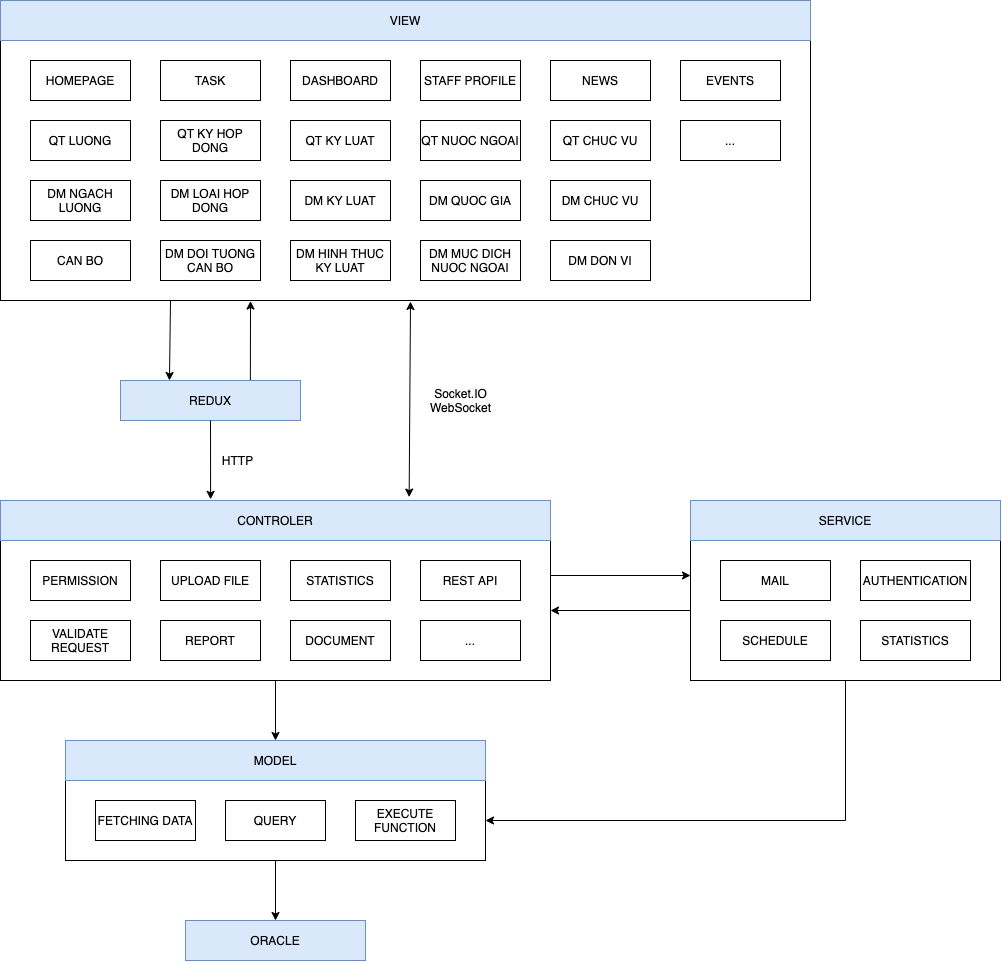
\includegraphics[width=15cm]{img/MVCInTchc.png}
  \captionof{figure}{Kiến trúc tổng thể của hệ thống}
\end{center}

\section{Cấu trúc cây thư mục của mã nguồn}
Việc cần làm đầu tiên và quan trọng nhất là tổ chức files và các thư mục. Với một thiết kế tốt thì khi làm việc chung giữa nhiều người sẽ ít bị đụng độ. Nhóm lựa chọn cách chia mỗi thành phần của trang ra từng module tách biệt với nhau, thuận lợi cho việc mở rộng và bảo trì, bảo dưỡng.\\

Dựa vào kiến trúc hệ thống mà nhóm đã thiết kế ở trên, nhóm đã thiết kế cấu trúc mã nguồn như sau:
\begin{center}
  \captionsetup{type=figure}
  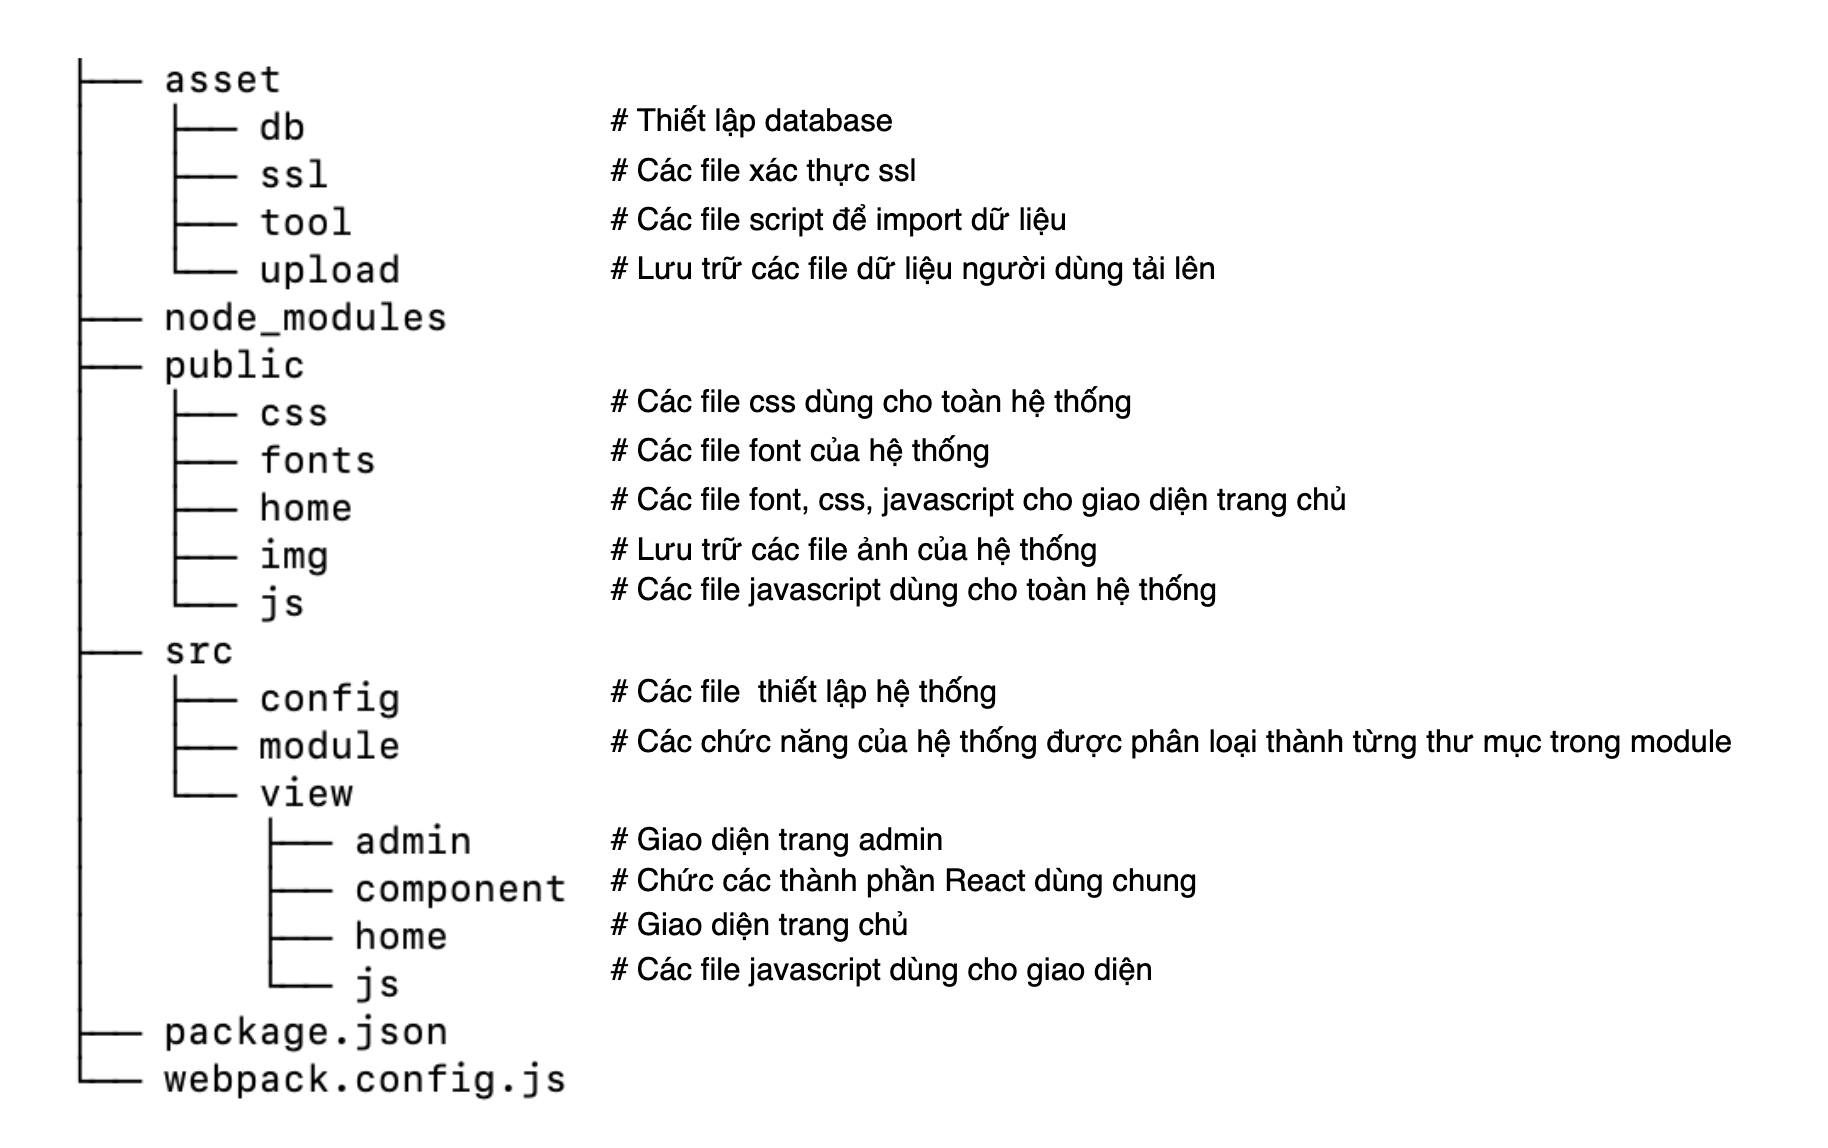
\includegraphics[width=15cm]{img/tree.png}
  \captionof{figure}{Cây thư mục của hệ thống}
\end{center}

Nhóm chia các danh mục, quá trình, chức năng vào từng module riêng, các module được thiết kế thống nhất theo mô hình MVC kết hợp với Redux. 

Cách chia module này thuận lợi cho phân chia công việc, tránh đụng độ trong phát triển hệ thống, dễ dàng thêm các module mới trong quá trình mở rộng, giúp cho việc tìm và sửa lỗi trong quá trình bảo trì trở nên đơn giản hơn.

\begin{figure}[H]
    \centering
    \begin{subfigure}[b]{0.4\linewidth}
        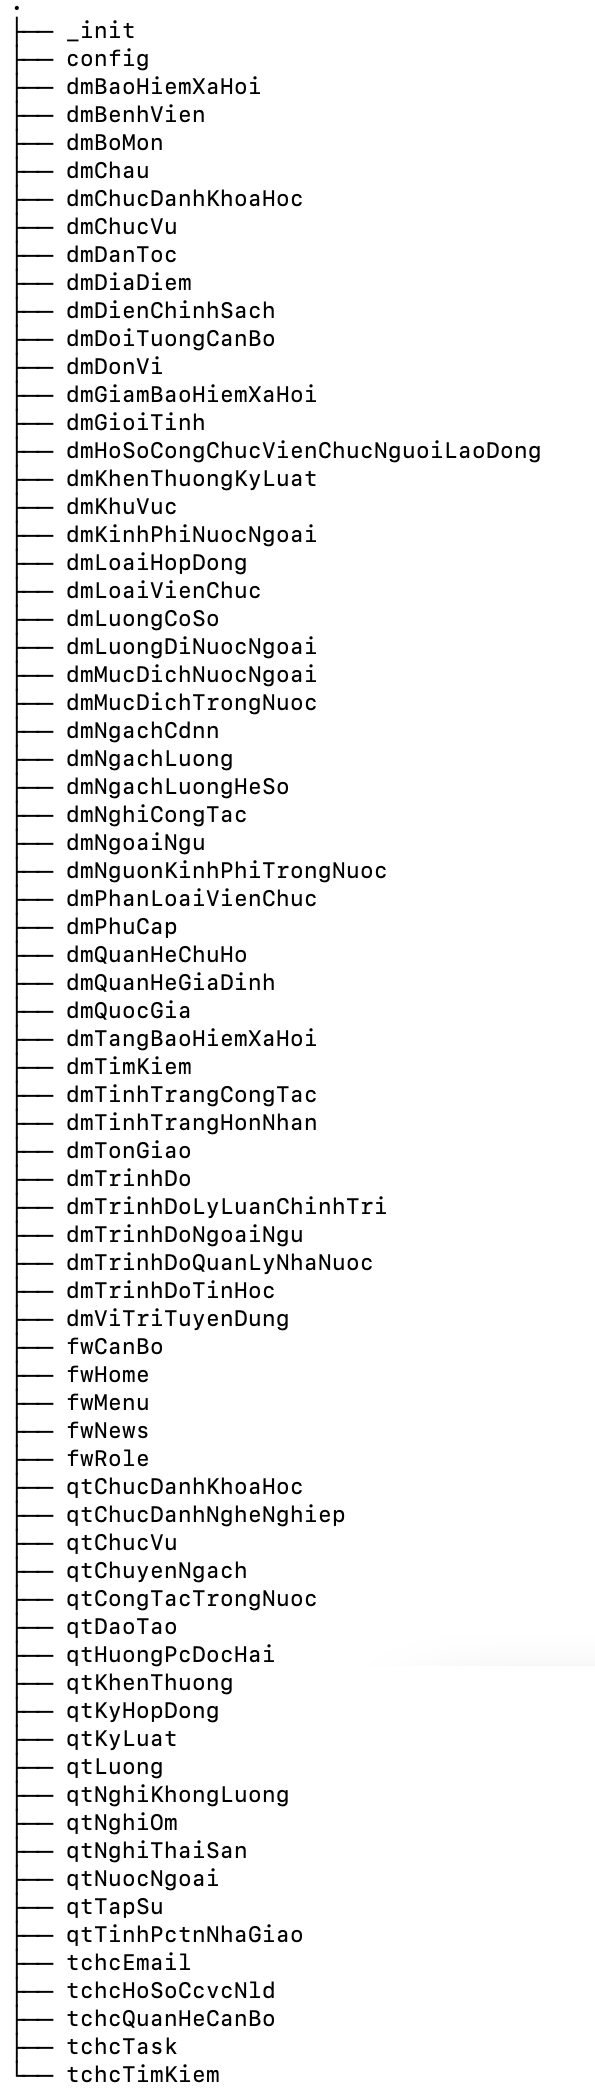
\includegraphics[width=\linewidth]{img/module.png}
        \caption{Thư mục module}
    \end{subfigure}
    \begin{subfigure}[b]{0.4\linewidth}
        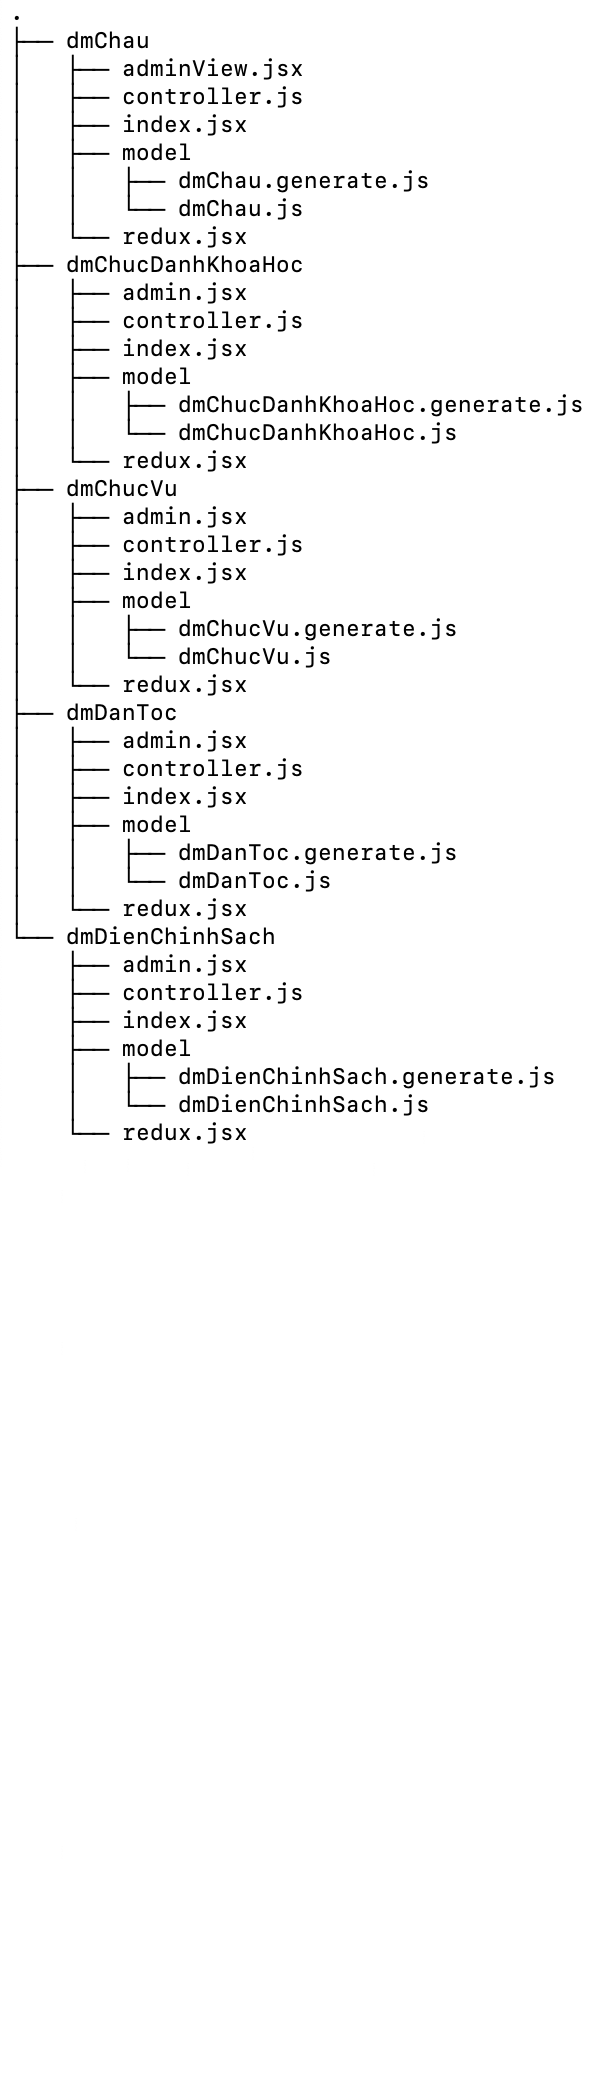
\includegraphics[width=\linewidth]{img/moduleDetail.png}
        \caption{Chi tiết từng module}
    \end{subfigure}
    \caption{Thư mục module của hệ thống}
\end{figure}





\section{Thiết kế đối tượng người dùng}
\subsection{Danh sách đối tượng người dùng}
\begin{center}
  \captionsetup{type=figure}
  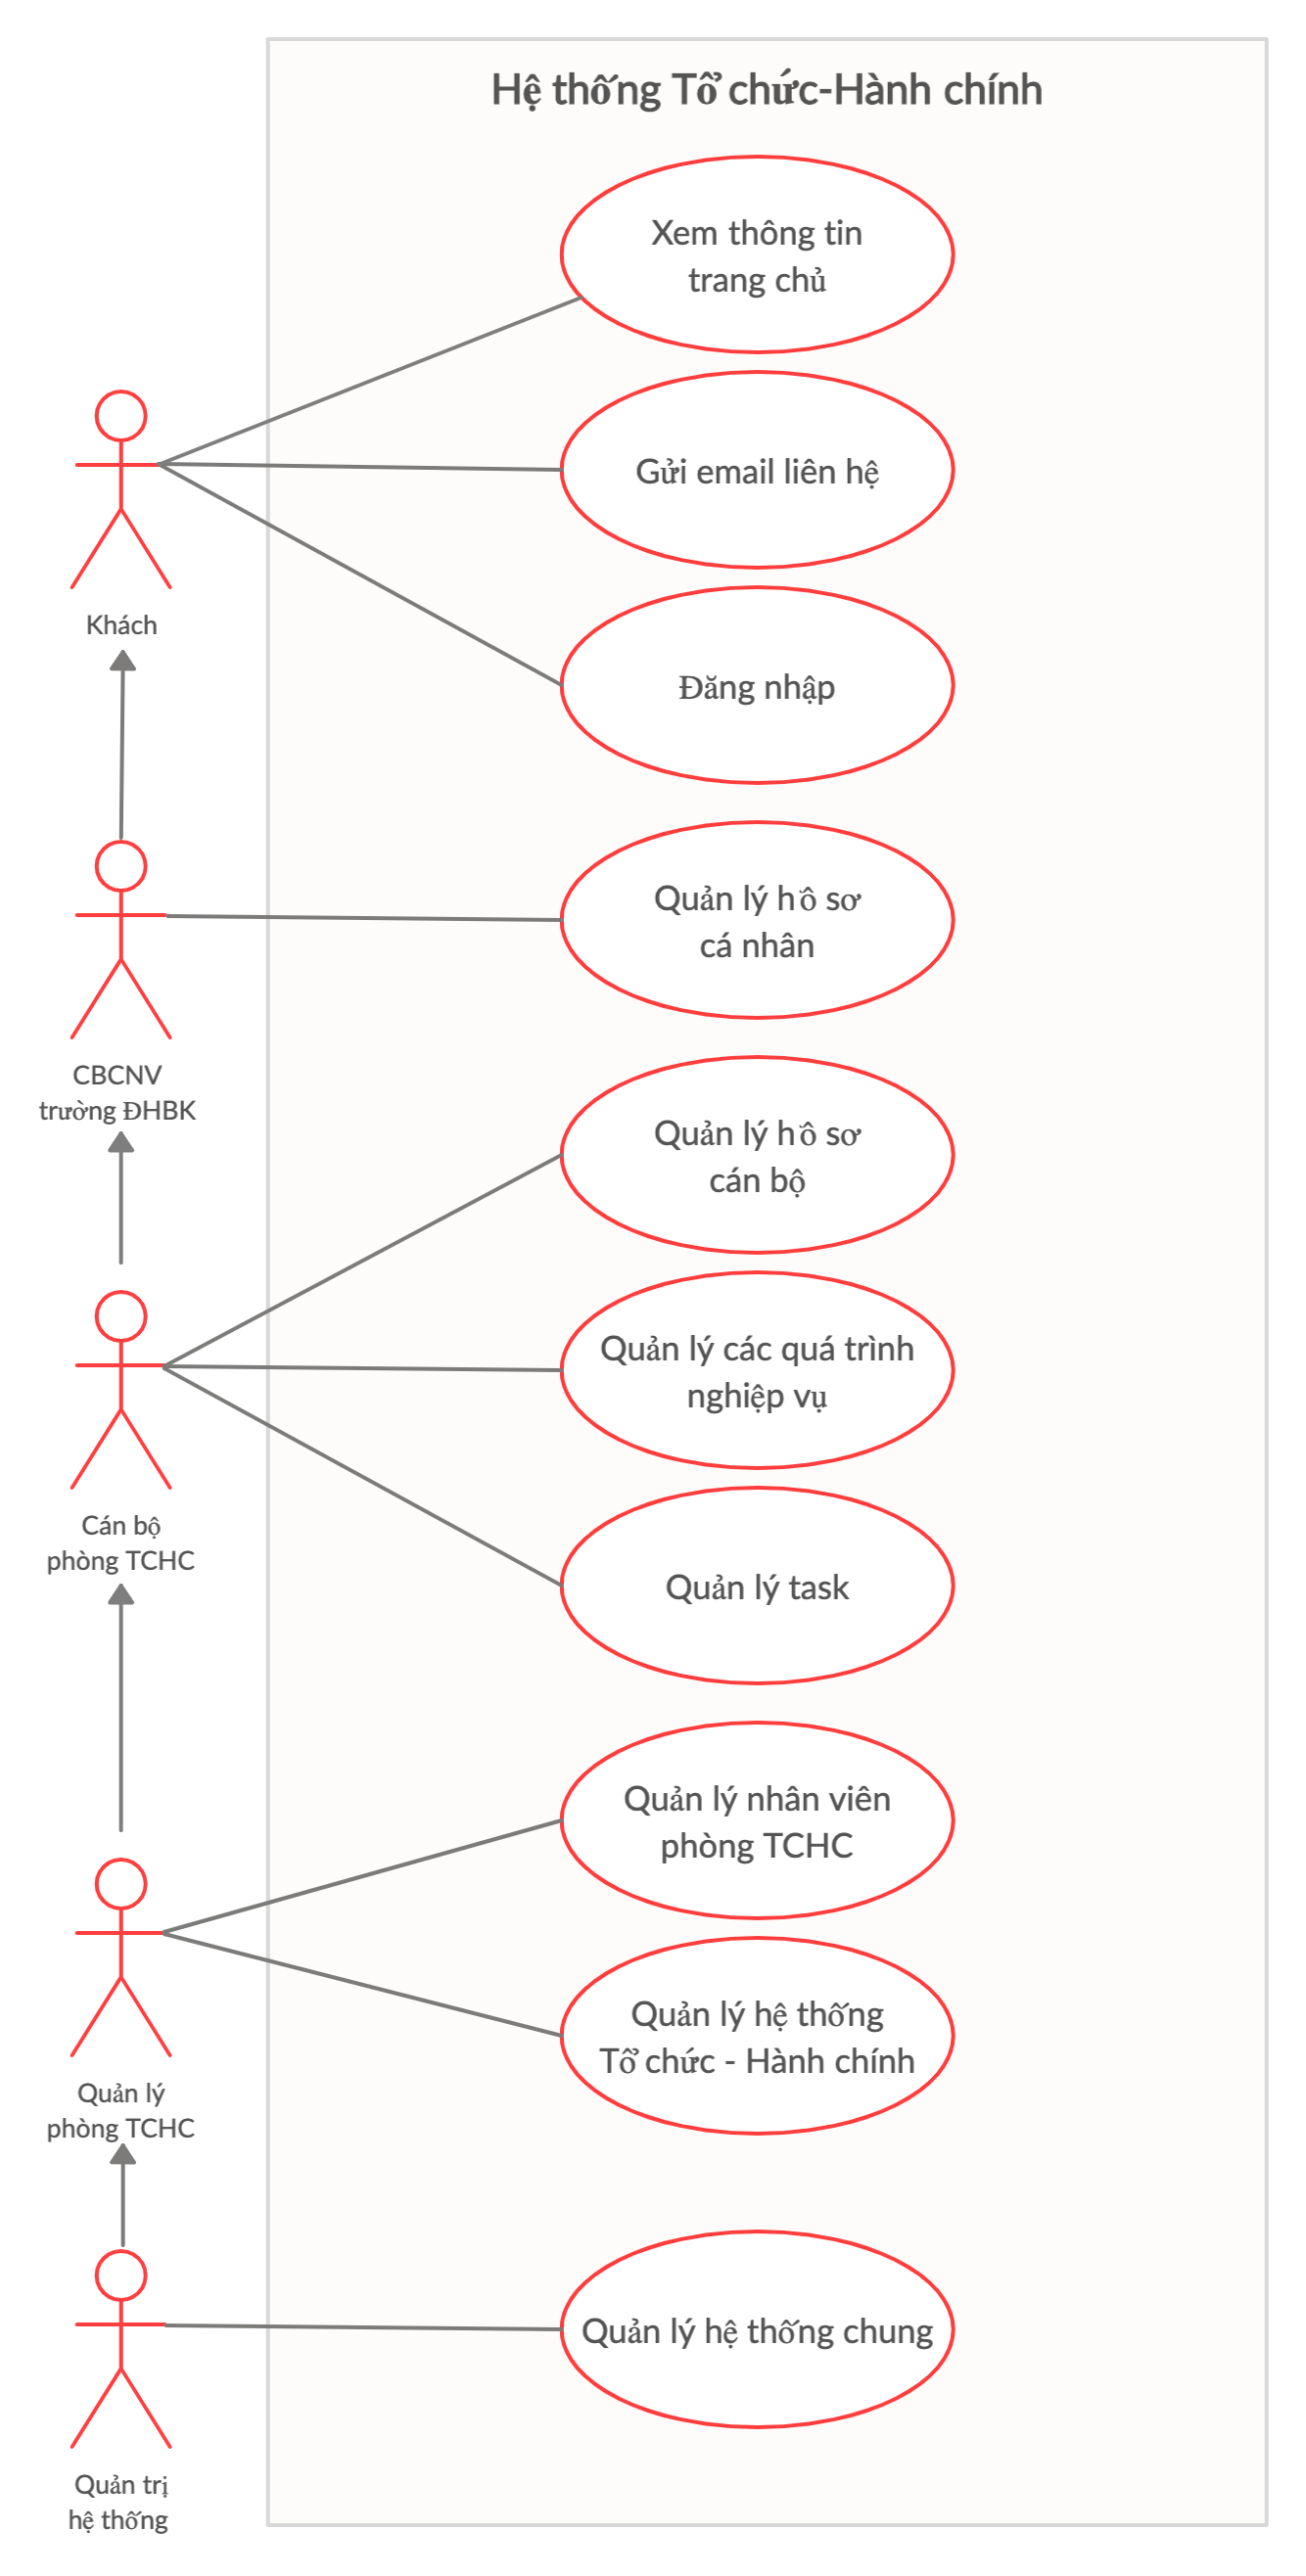
\includegraphics[width=11cm]{img/usecase/rootUsecase.png}
  \captionof{figure}{Lược đồ Usecase các đối tượng của hệ thống }
\end{center}
\begin{table}[H]
    \centering
	\begin{tabular}{|p{1cm}|p{4cm}|p{10cm}|}
    \hline
    \textbf{STT}&\textbf{Người dùng}&\textbf{Đặc tả}\\
    \hline
    1&Khách&Là những người dùng chưa đăng nhập, bao gồm tất cả các đối tượng như cán bộ công nhân viên nhà trường, sinh viên, cựu sinh viên, phụ huynh, đơn vị, doanh nghiệp là đối tác của nhà trường,...
    
    Khách có chức năng xem thông tin, tin tức, sự kiện của nhà trường, gửi email liên hệ, và đăng nhập.\\
    \hline
	2&Cán bộ công nhân viên nhà trường&Người dùng với mục đích quản lý được thông tin, hồ sơ, các quá trình nghiệp vụ của bản thân.\\
	\hline
    3&Cán bộ phòng Tổ chức - Hành chính&Là những cán bộ thuộc phòng Tổ chức - Hành chính. Họ có chức năng quản lý thông tin của các cán bộ, quản lý thông tin các quá trình nghiệp vụ của nhà trường.\\
    \hline
    4&Quản lý phòng Tổ chức - Hành chính (Trưởng phòng, phó phòng) &Chức năng chính là quản lý hệ thống và công việc của các cán bộ thuộc phòng Tổ chức - Hành chính. \\
	\hline
    5&Quản trị hệ thống&Là những người tạo ra hệ thống ban đầu, có các chức năng hỗ trợ tạo ra các cấu hình cho hệ thống, bao gồm các thao tác như: cấu hình các thông tin chung của phòng Tổ chức-Hành chính, cấu hình về giao diện, quản lý tài khoản người dùng\\
	\hline
\end{tabular}
\caption{Danh sách đối tượng người dùng của hệ thống}
\end{table}
\subsection{Đối tượng: Khách}
\textbf{Lược đồ Usecase đối tượng khách}
\begin{center}
  \captionsetup{type=figure}
  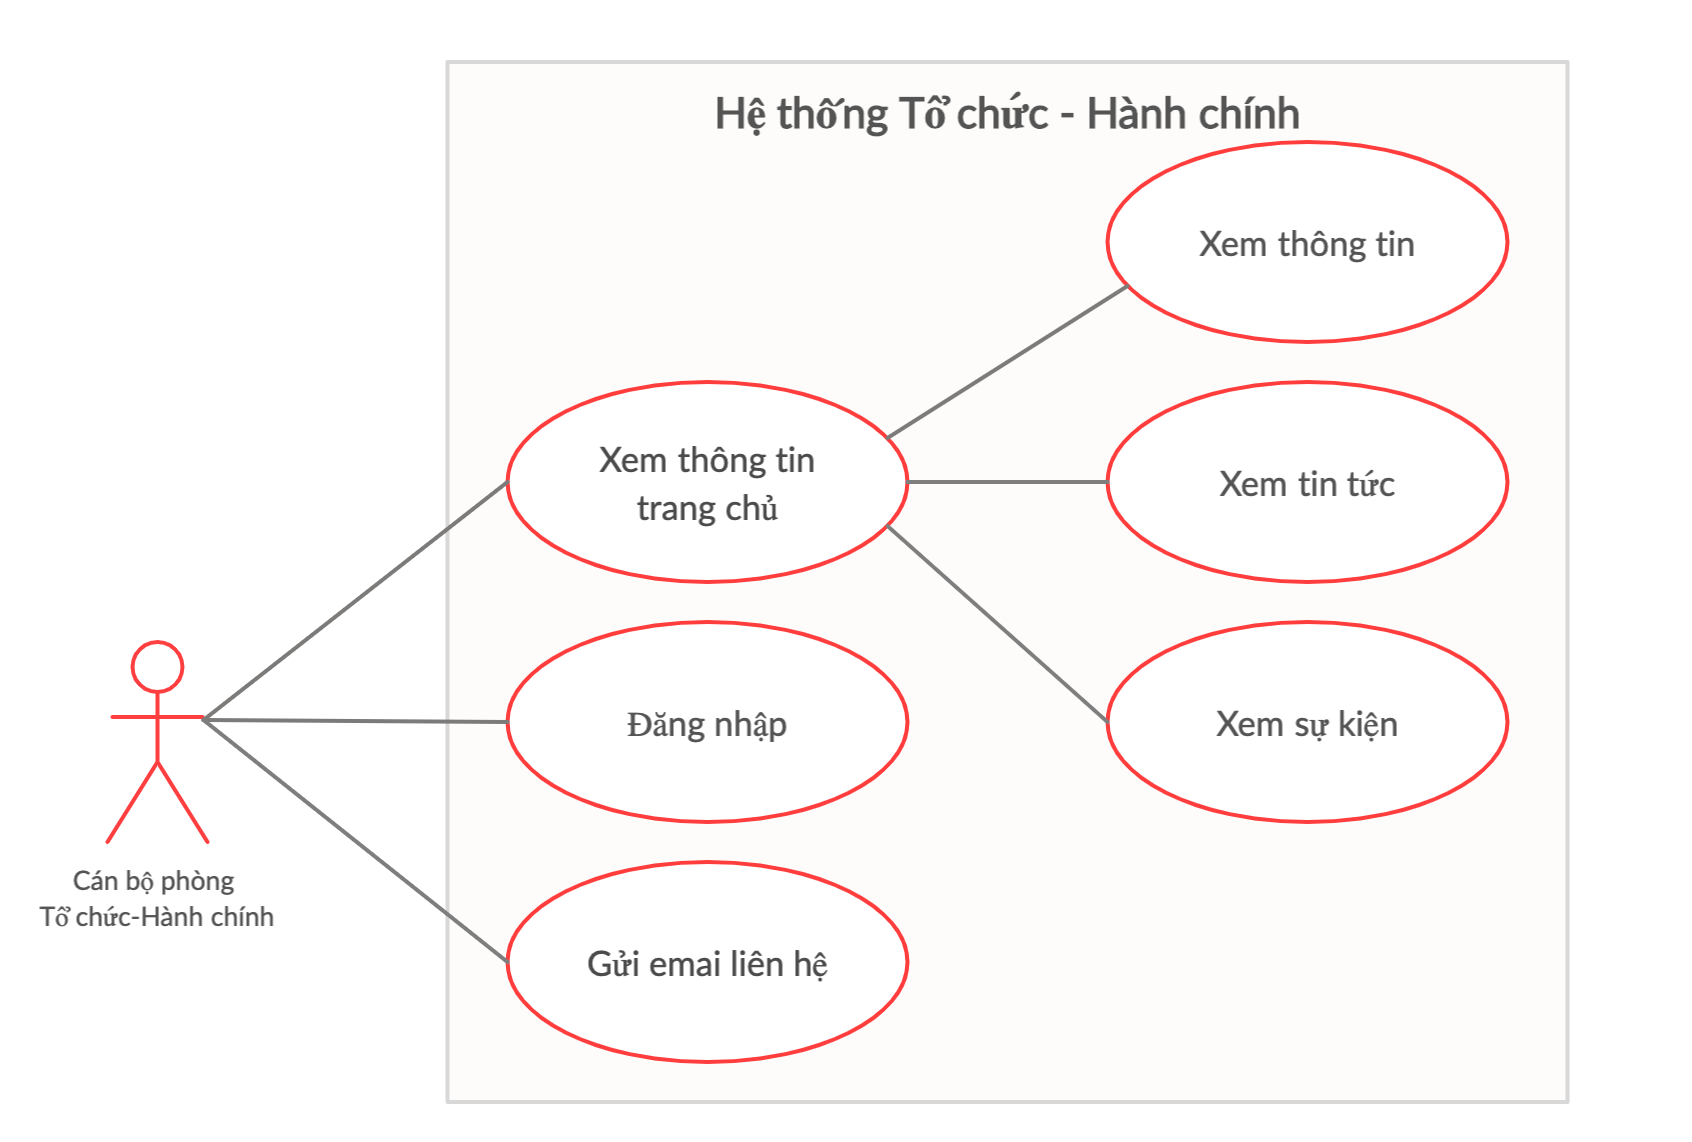
\includegraphics[width=14cm]{img/usecase/guest.png}
  \captionof{figure}{Lược đồ Usecase của đối tượng khách}
\end{center}

Khách là những người dùng chưa đăng nhập, bao gồm tất cả các đối tượng như cán bộ công nhân viên nhà trường, sinh viên, cựu sinh viên, phụ huynh, đơn vị, doanh nghiệp là đối tác của nhà trường,...
 
 Đối tượng khách có thể truy cập trang chủ để xem các thông tin chung, thông tin liên hệ, xem các tin tức và sự kiện. Khi có nhu cầu liên hệ với nhà trường, khách có thể vào mục liên hệ để gửi email đến nhà trường.
 
 Khi khách là cán bộ công nhân viên trường Đại học Bách Khoa Tp.HCM, khách có thể đăng nhập bằng tài khoản email nhà trường cung cấp để sử dụng hệ thống với các vai trò cán bộ nhà trường.

\subsection{Đối tượng: Cán bộ công nhân viên nhà trường}
\textbf{Lược đồ Usecase đối tượng cán bộ của trường}
\begin{center}
  \captionsetup{type=figure}
  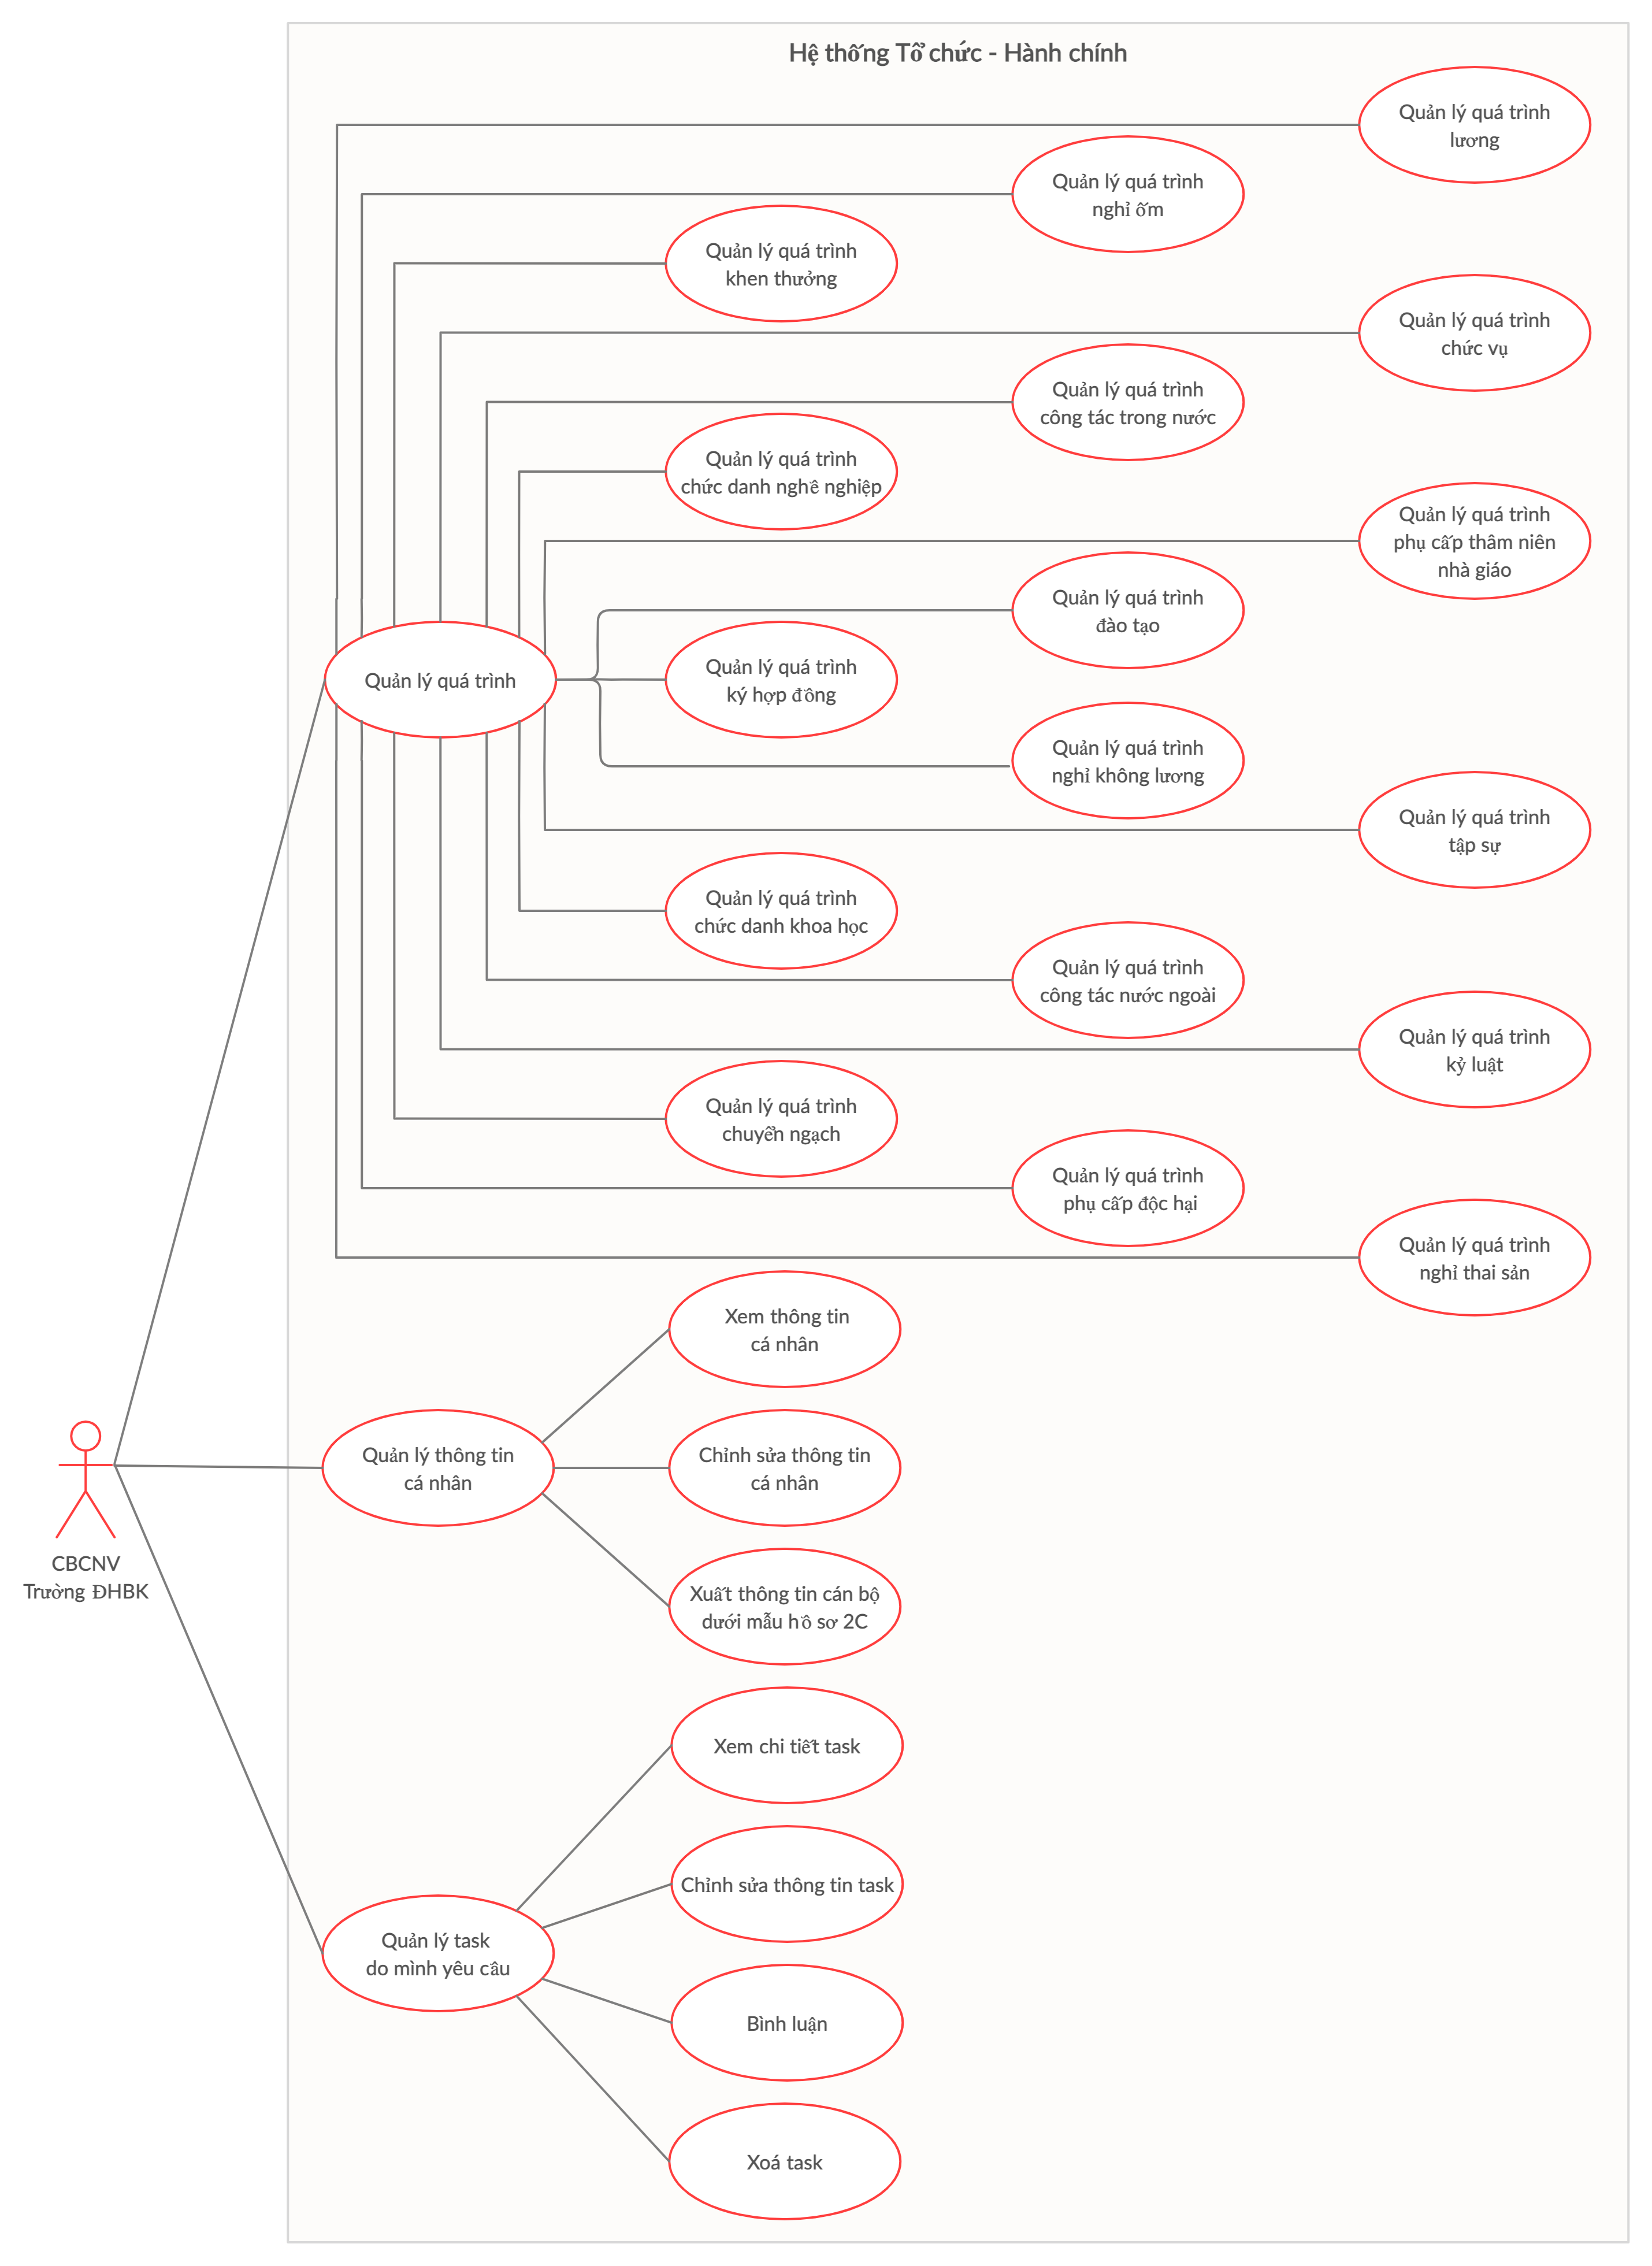
\includegraphics[width=15cm]{img/usecase/userUsecase.png}
  \captionof{figure}{Lược đồ Usecase đối tượng cán bộ công nhân viên nhà trường}
\end{center}

Đối với người dùng là cán bộ của trường, sau khi đăng nhập sẽ có chức năng quản lý thông tin của cá nhân, quản lý các quá trình nghiệp vụ của bản thân.

Quản lý thông tin cá nhân bao gồm xem thông tin, sửa đổi và xuất thông tin theo mẫu sơ yếu lý lịch cán bộ, công chức (Mẫu 2C-BNV/2008).

Cán bộ có thể xem thông tin các quá trình nghiệp vụ của bản thân như quá trình lương, quá trình nghỉ ốm, nghỉ không lương, nghỉ thai sản,... 

Khi muốn tạo mới, sửa đổi hoặc xoá quá trình, cán bộ công nhân viên nhà trường có thể tạo yêu cầu tương ứng để cán bộ phòng Tổ chức - Hành chính xem xét và duyệt yêu cầu.

\subsection{Đối tượng: Cán bộ phòng Tổ chức - Hành chính}
\textbf{Lược đồ Usecase đối tượng cán bộ phòng Tổ chức - Hành chính}
\begin{center}
  \captionsetup{type=figure}
  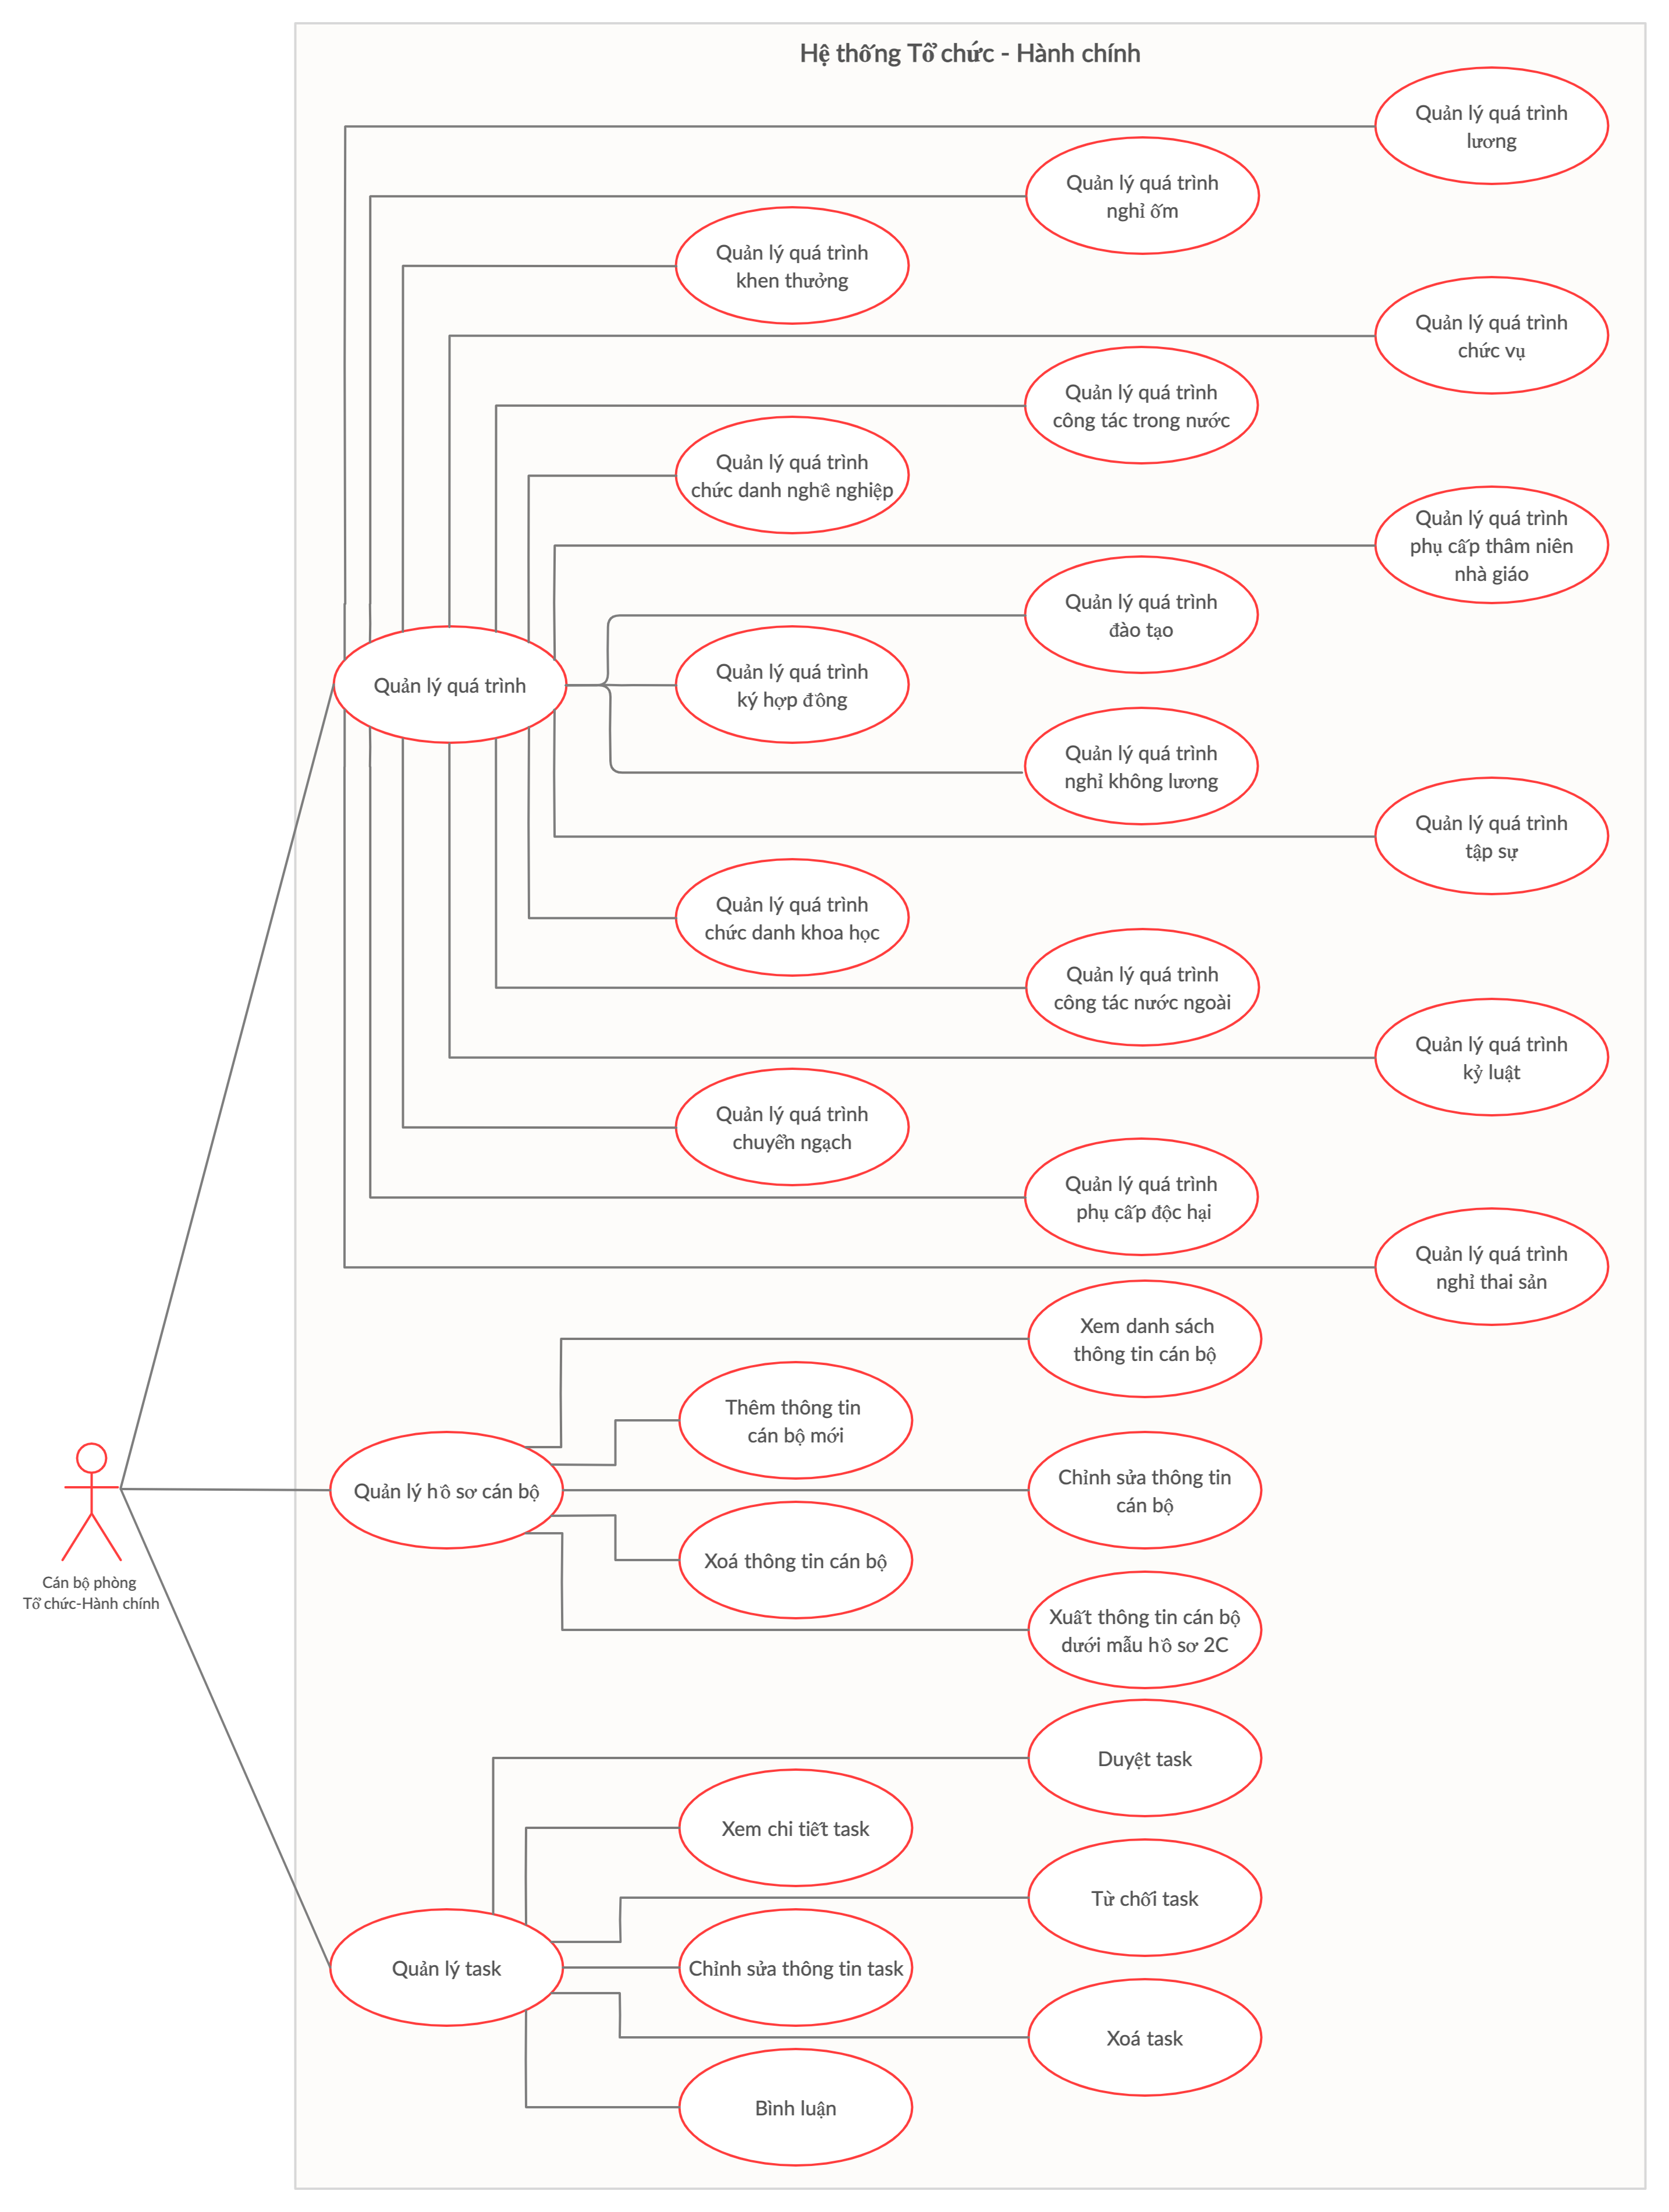
\includegraphics[width=15cm]{img/usecase/nhanVienTCHC.png}
  \captionof{figure}{Lược đồ Usecase đối tượng cán bộ phòng Tổ chức - Hành chính}
\end{center}

Sau khi đăng nhập vào hệ thống, người dùng là cán bộ phòng Tổ chức - Hành chính sẽ có các nhóm chức năng sau: quản lý cán bộ, quản lý các quá trình nghiệp vụ và các yêu cầu của của người dùng.

Chức năng quản lý cán bộ bao gồm xem danh sách toàn bộ cán bộ nhà trường, tạo mới, sửa đổi và xoá cán bộ. Ngoài ra còn có chức năng xuất danh sách cán bộ dưới dạng excel, xuất hồ sơ lý lịch theo mẫu 2C.

Chức năng quản lý các quá trình nghiệp vụ bao gồm xem danh sách các quá trình như quá trình công tác trong nước, quá trình công tác nước ngoài, quá trình lương,... Tạo mới quá trình, chỉnh sửa thông tin quá trình và xoá quá trình.

Cán bộ phòng Tổ chức - Hành chính còn có nhiệm vụ quản lý các yêu cầu của các cán bộ công nhân viên nhà trường, xem xét, chỉnh sửa, bình luận, từ chối và duyệt yêu cầu.

\subsection{Đối tượng: Quản lý phòng Tổ chức - Hành chính}
\textbf{Lược đồ Usecase đối tượng quản lý phòng Tổ chức - Hành chính}
\begin{center}
  \captionsetup{type=figure}
  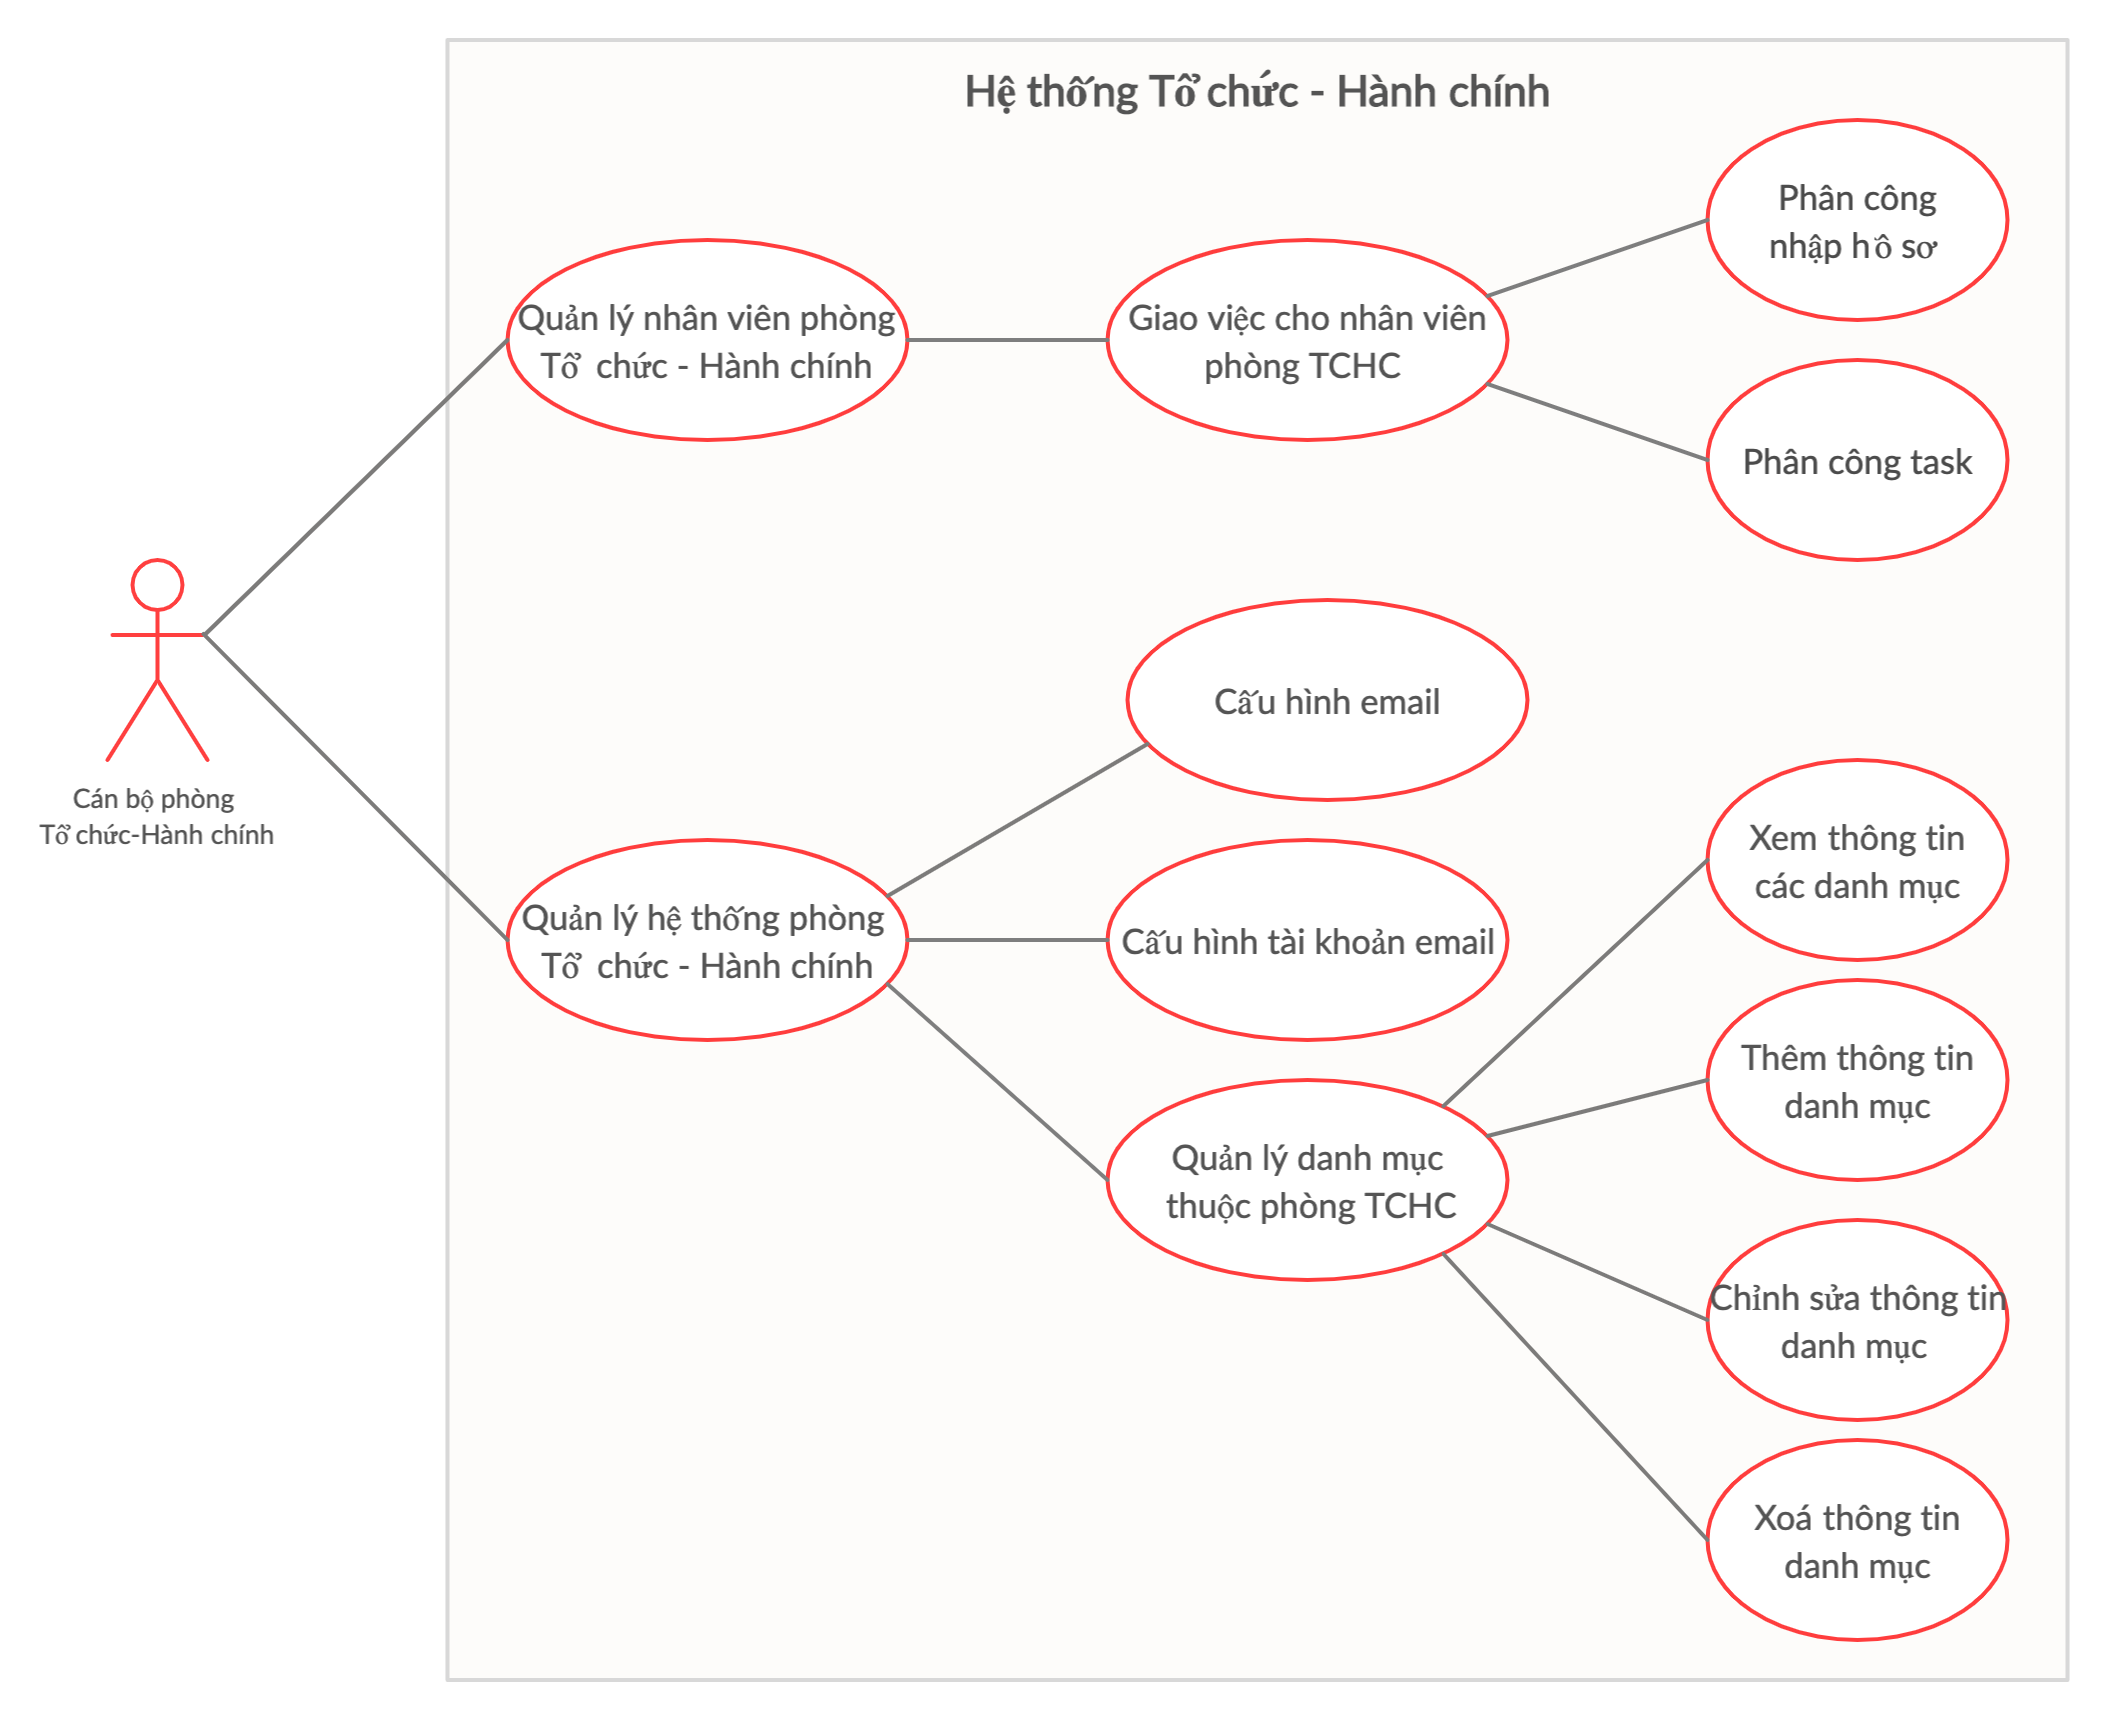
\includegraphics[width=15cm]{img/usecase/quanLyPhong.png}
  \captionof{figure}{Lược đồ Usecase cho đối tượng quản lý phòng Tổ chức - Hành chính}
\end{center}
Quản lý phòng Tổ chức - Hành chính sau khi đăng nhập sẽ có tất cả các nhóm chức năng như trên của cán bộ của phòng Tổ chức - Hành chính và có thêm chức năng quản trị các danh mục, thông tin thuộc phòng Tổ chức - Hành chính.

Bên cạnh đó, quản lý phòng còn có nhiệm vụ phân công công việc cho nhân viên như phân công nhập hồ sơ, phân công duyệt yêu cầu.

\subsection{Đối tượng: Quản trị hệ thống}
\textbf{Lược đồ Usecase đối tượng quản trị hệ thống}
\begin{center}
  \captionsetup{type=figure}
  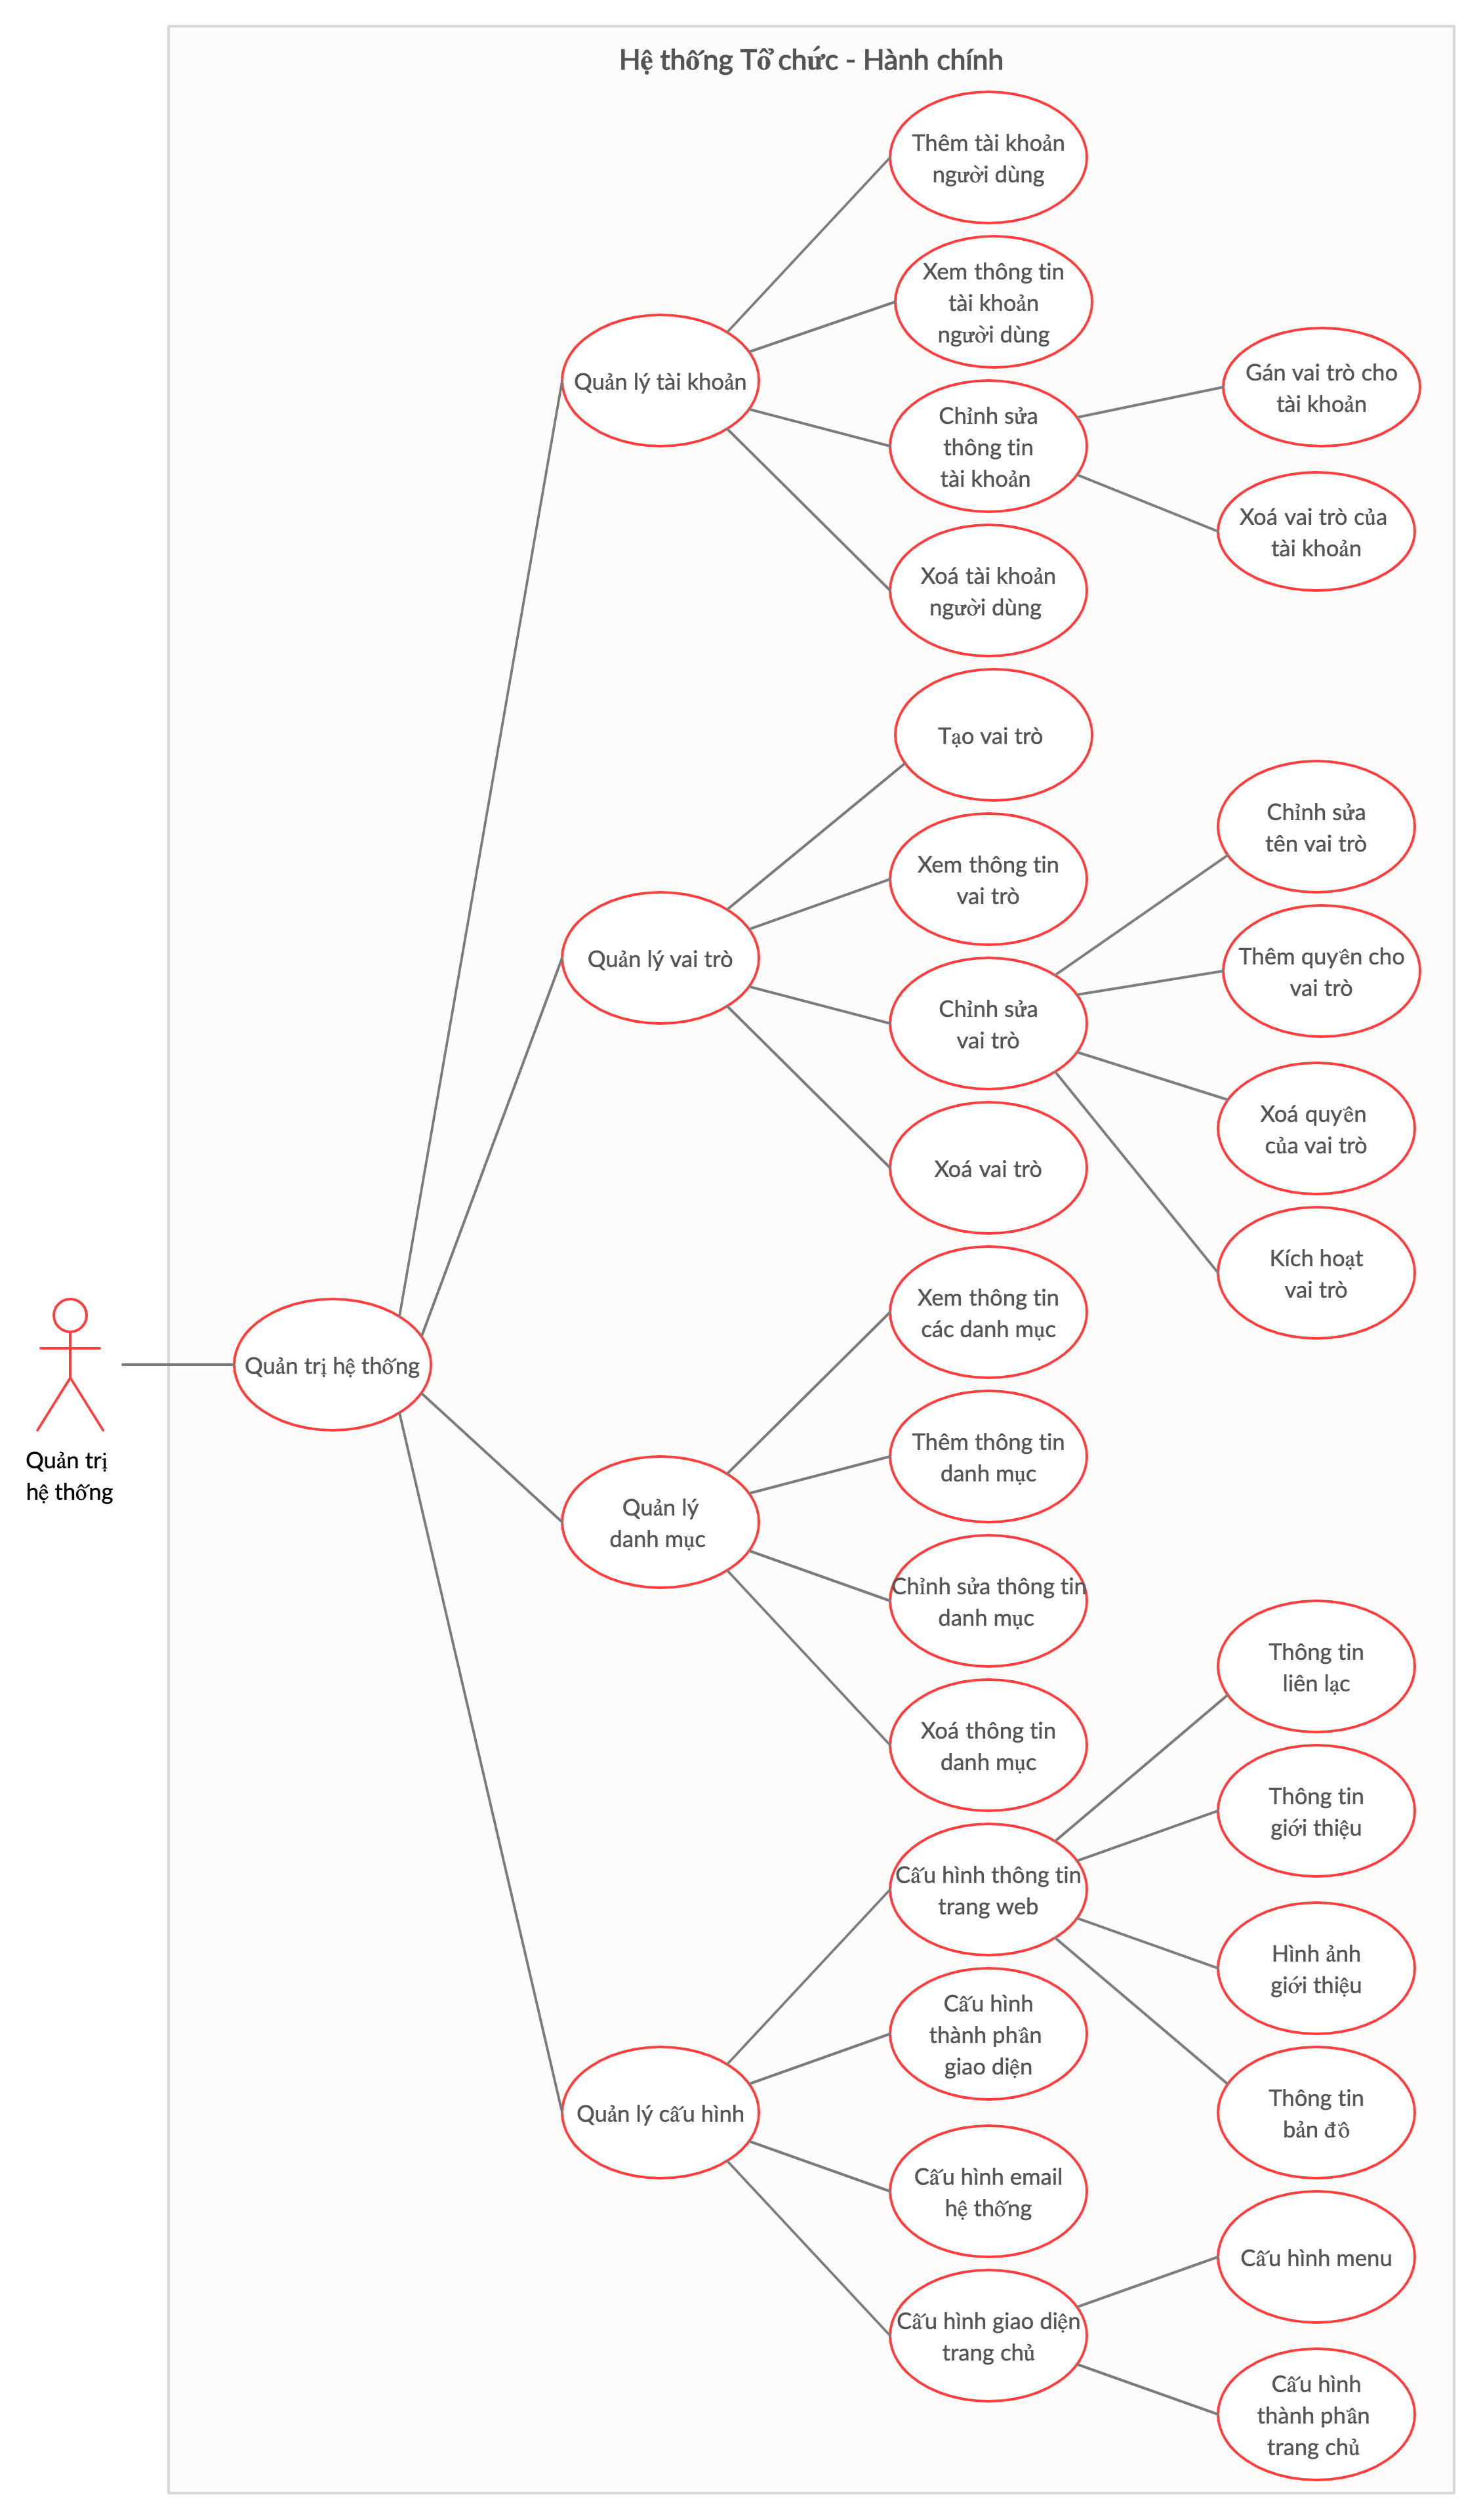
\includegraphics[width=13cm]{img/usecase/admin.png}
  \captionof{figure}{Lược đồ usecase của đối tượng quản trị hệ thống}
\end{center}

\indent Đối với đối tượng là quản trị hệ thống, sau khi xác thực thành công sẽ có những nhóm chức năng: quản lý tài khoản, quản lý vai trò, quản lý danh mục và quản lý cấu hình. Với mỗi nhóm chức năng sẽ có những chức năng tương ứng sau:

\begin{itemize}
    \item Nhóm quản lý tài khoản bao gồm các chức năng:
        \subitem - Xem thông tin các tài khoản.
        \subitem - Tạo mới tài khoản.
        \subitem - Xoá tài khoản người dùng.
        \subitem - Chỉnh sửa thông tin tài khoản.
        \subitem - Thêm và xoá vai trò cho tài khoản.
    \item Nhóm quản lý vai trò bao gồm các chức năng:
        \subitem - Xem danh sách các vai trò.
        \subitem - Tạo mới và xoá vai trò.
        \subitem - Kích hoạt vai trò.
        \subitem - Thêm và xoá quyền cho vai trò.
    \item Chức năng quản lý danh mục là chức năng xây dựng và sửa đổi thông tin những danh mục mặc định phục vụ cho việc nhập và lữu trữ dữ liệu trong hệ thống.
    \item Nhóm quản lý cấu hình gồm các chức năng: cấu hình giao diện trang chủ, cấu hình thông tin trang web, cấu hình email cho hệ thống.
        \subitem - Cấu hình giao diện trang chủ: Tùy chỉnh các thành phần giao diện, lựa chọn các thành phần giao diện sẽ xuất hiện ở trang chủ.
        \subitem - Cấu hình thông tin trang web: Cấu hình các thông tin chung cho hệ thống, thông tin liên lạc của phòng Tổ chức - Hành chính.
        \subitem - Cấu hình email hệ thống: Tủy chỉnh các mẫu email tự động của hệ thống.
\end{itemize}
\newpage
\section{Thiết kế cơ sở dữ liệu cho hệ thống}
\begin{center}
  \captionsetup{type=figure}
  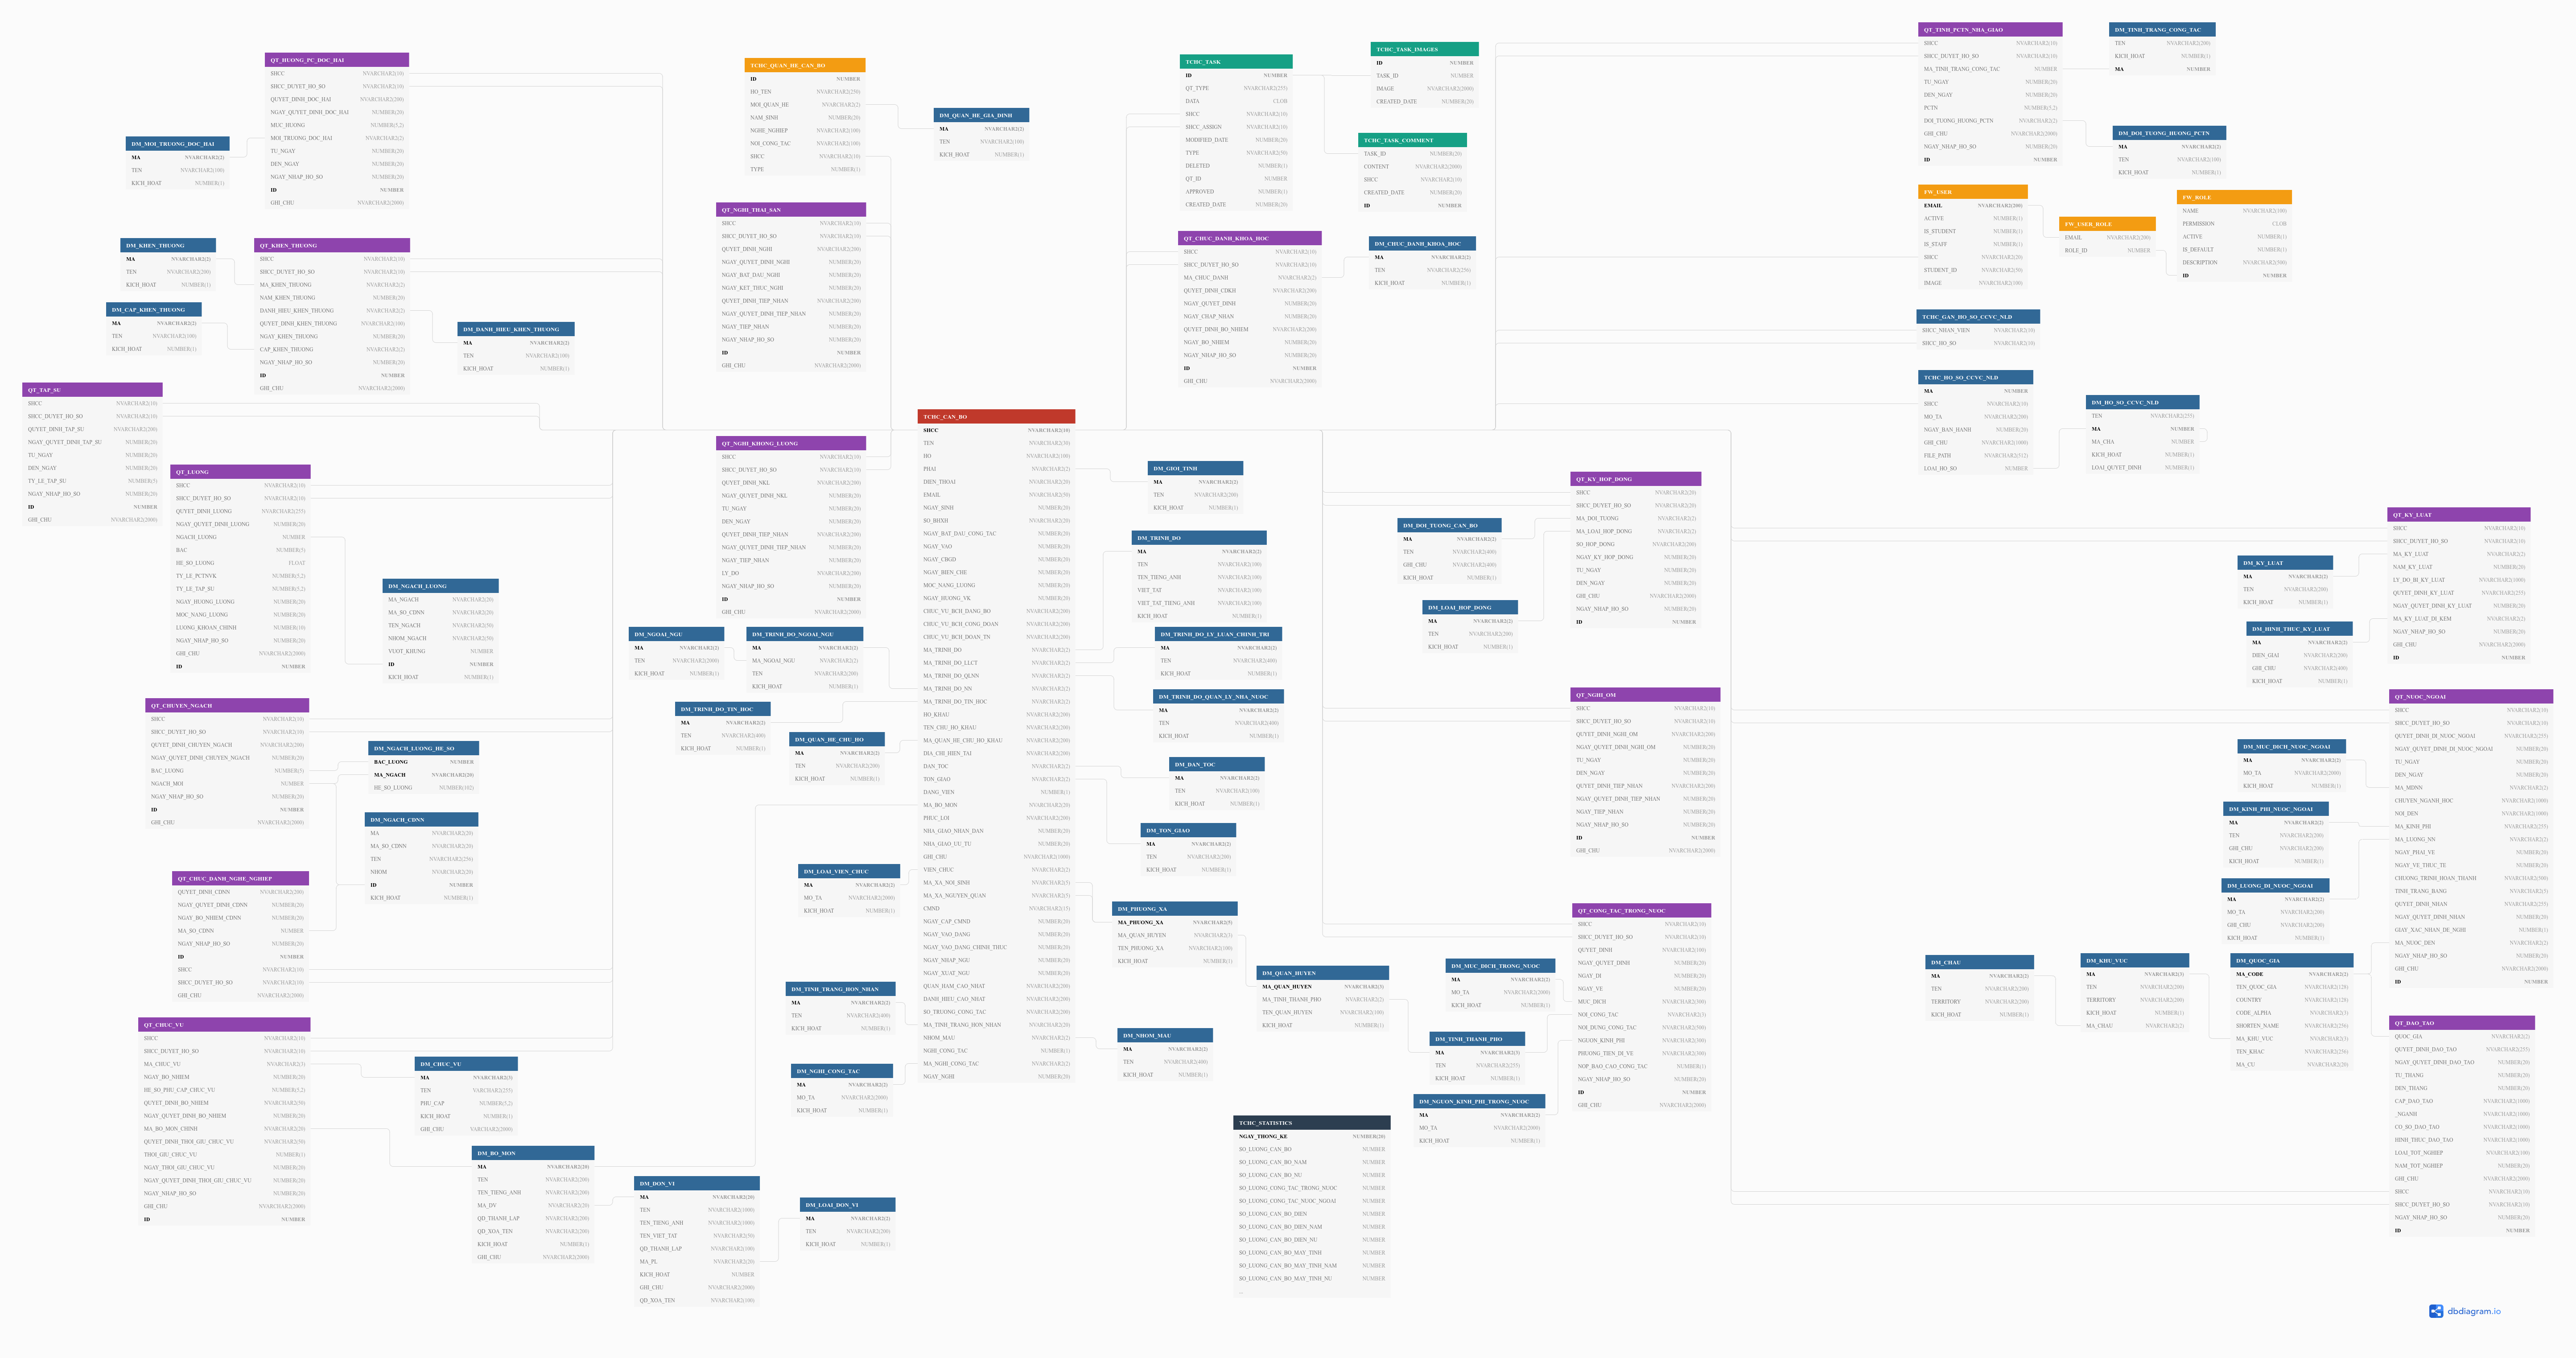
\includegraphics[width=15cm]{img/Screen/dbdiagram.png}
  \captionof{figure}{Thiết kế cơ sở dữ liệu của hệ thống}
\end{center}
Chi tiết xem ở tài liệu đính kèm.
% \newpage
